\documentclass[11pt,a4paper]{article}
\usepackage[utf8]{inputenc}
\usepackage[T1]{fontenc}
\usepackage[scaled=0.92]{helvet}
\renewcommand{\familydefault}{\sfdefault}
\usepackage[a4paper,margin=2.3cm,headheight=14pt]{geometry}
\usepackage{microtype}
\usepackage[table]{xcolor}
\usepackage{graphicx,booktabs,tabularx,longtable,array,enumitem,parskip,float,caption,multirow}
\usepackage{fancyhdr,titlesec}
\usepackage[most]{tcolorbox}
\usepackage{tikz}
\usetikzlibrary{arrows.meta,positioning,shapes.geometric}
\usepackage{listings}
\usepackage[hidelinks]{hyperref}

\definecolor{navy}{HTML}{1F2A44}
\definecolor{ermgreen}{HTML}{2E7D32}
\definecolor{ermamber}{HTML}{F9A825}
\definecolor{ermred}{HTML}{C62828}
\definecolor{tintgreen}{HTML}{C8E6C9}
\definecolor{tintamber}{HTML}{FFF3C4}
\definecolor{tintred}{HTML}{F8CACA}
\definecolor{softgrey}{HTML}{F2F4F7}
\definecolor{inputblue}{HTML}{0000FF}
\definecolor{linkgreen}{HTML}{008000}

\hypersetup{colorlinks=true,linkcolor=navy,urlcolor=navy,citecolor=navy,
  pdftitle={Panduan Penggunaan ERM Framework ASB},pdfauthor={ERM Framework (portfolio project)}}

\titleformat{\section}{\Large\bfseries\color{navy}}{\thesection}{0.8em}{}[{\color{navy}\titlerule[0.8pt]}]
\titleformat{\subsection}{\large\bfseries\color{navy}}{\thesubsection}{0.6em}{}
\titleformat{\subsubsection}{\normalsize\bfseries\color{navy}}{\thesubsubsection}{0.5em}{}
\titlespacing*{\section}{0pt}{1.4em}{0.8em}

\pagestyle{fancy}
\fancyhf{}
\fancyhead[L]{\small\color{gray}Panduan Penggunaan --- ERM Framework PT Amanah Syariah Bank (fiktif)}
\fancyfoot[L]{\small\color{gray}Bank fiktif \textbullet{} data sintetis}
\fancyfoot[R]{\small\color{gray}Halaman \thepage}
\renewcommand{\headrulewidth}{0.4pt}

\renewcommand{\contentsname}{Daftar Isi}
\renewcommand{\figurename}{Gambar}
\renewcommand{\tablename}{Tabel}
\setlist[itemize]{topsep=2pt,itemsep=2pt}
\setlist[enumerate]{topsep=2pt,itemsep=3pt}
\setlength{\LTpre}{4pt}\setlength{\LTpost}{6pt}
\renewcommand{\arraystretch}{1.25}

\newtcolorbox{tipbox}[1][Tips]{colback=tintgreen!45,colframe=ermgreen,fonttitle=\bfseries,title=#1,boxrule=0.6pt,arc=2pt,left=6pt,right=6pt}
\newtcolorbox{warnbox}[1][Perhatian]{colback=tintamber!60,colframe=ermamber!90!black,coltitle=black,fonttitle=\bfseries,title=#1,boxrule=0.6pt,arc=2pt,left=6pt,right=6pt}
\newtcolorbox{infobox}[1][Catatan]{colback=softgrey,colframe=navy,fonttitle=\bfseries,title=#1,boxrule=0.6pt,arc=2pt,left=6pt,right=6pt}
\newtcolorbox{stepbox}[1]{colback=white,colframe=navy!70,fonttitle=\bfseries,title=#1,boxrule=0.5pt,arc=2pt,left=6pt,right=6pt}

\lstset{basicstyle=\ttfamily\small,backgroundcolor=\color{softgrey},frame=single,rulecolor=\color{gray!40},
  columns=fullflexible,keepspaces=true,breaklines=true,xleftmargin=4pt,xrightmargin=4pt,aboveskip=6pt,belowskip=6pt,
  literate={-}{-}1}
\newcommand{\file}[1]{\texttt{\small #1}}
\newcommand{\tagG}{\colorbox{tintgreen}{\strut Hijau}}
\newcommand{\tagA}{\colorbox{tintamber}{\strut Kuning}}
\newcommand{\tagR}{\colorbox{tintred}{\strut Merah}}

\begin{document}
\sloppy
\begin{titlepage}
\thispagestyle{empty}
\vspace*{2.2cm}
{\color{navy}\rule{\linewidth}{2pt}}\\[1.2em]
{\Huge\bfseries\color{navy} Panduan Penggunaan}\\[0.6em]
{\LARGE\color{navy} Enterprise Risk Management Framework\\[0.2em] untuk Bank Syariah}\\[1.2em]
{\large PT Amanah Syariah Bank (fiktif) \textbullet{} Risk Appetite, Monitoring \& Stress Testing}\\[0.8em]
{\color{navy}\rule{\linewidth}{0.8pt}}
\vspace{1.6cm}

\begin{tcolorbox}[colback=softgrey,colframe=navy,boxrule=0.6pt,arc=2pt,left=10pt,right=10pt,top=8pt,bottom=8pt]
\textbf{Isi paket yang dibahas:} \file{erm\_\allowbreak{}final.zip} (folder \file{enterprise-risk-management})\\[0.3em]
\textbf{Posisi data:} September 2026 \textbullet{} \textbf{Periode:} Oktober 2025 -- September 2026\\[0.3em]
\textbf{Untuk siapa:} pembaca non-programmer yang ingin membuka, menjalankan, membaca, dan menjelaskan project ini\\[0.3em]
\textbf{Status regulasi diperiksa per:} 2026-09-17
\end{tcolorbox}

\vfill
{\small\color{gray}
\textbf{Disclaimer.} This project uses a fictional Islamic bank and fully synthetic data. All risk appetite thresholds, scenarios, sensitivities, and scoring rules are project-specific analytical assumptions created for educational and portfolio purposes. They do not represent any actual bank's internal limits, regulatory thresholds, or an official OJK risk profile rating.}
\end{titlepage}

\tableofcontents
\newpage
\section{Tentang Panduan Ini}

Panduan ini menjelaskan cara memakai project \emph{Enterprise Risk Management (ERM) Framework} untuk bank syariah fiktif \textbf{PT Amanah Syariah Bank (ASB)}. Bahasanya sengaja dibuat sederhana. Anda tidak perlu bisa memrogram untuk mengikuti sebagian besar isinya.

\subsection*{Pilih jalur yang sesuai kebutuhan Anda}

\begin{center}
\begin{tabularx}{\linewidth}{>{\bfseries}p{4.6cm}X}
\toprule
Kebutuhan & Bagian yang dibaca \\
\midrule
Hanya ingin melihat hasil & Bagian \ref{sec:overview}, \ref{sec:zip}, dan \ref{sec:quick} (tanpa instalasi apa pun) \\
Ingin menjelaskan project saat interview & Bagian \ref{sec:overview}, \ref{sec:istilah}, \ref{sec:report}, \ref{sec:stress}, dan \ref{sec:batasan} \\
Ingin menjalankan ulang di komputer sendiri & Bagian \ref{sec:persiapan}, \ref{sec:jalankan}, dan \ref{sec:test} \\
Ingin mencoba mengubah asumsi & Bagian \ref{sec:ubah} dan \ref{sec:masalah} \\
Ingin merakit dashboard Power BI & Bagian \ref{sec:powerbi} \\
\bottomrule
\end{tabularx}
\end{center}

\subsection*{Tanda yang dipakai dalam panduan}

\begin{tipbox}
Kotak hijau berisi saran yang memudahkan pekerjaan.
\end{tipbox}
\begin{warnbox}
Kotak kuning berisi hal yang perlu diperhatikan agar hasil tidak rusak atau salah dibaca.
\end{warnbox}
\begin{infobox}
Kotak abu-abu berisi penjelasan tambahan yang boleh dilewati.
\end{infobox}

Nama file dan folder ditulis dengan huruf seperti \file{data/output/kri\_\allowbreak{}monthly.csv}. Perintah yang diketik di komputer ditampilkan dalam kotak abu-abu seperti ini:
\begin{lstlisting}
python run_all.py
\end{lstlisting}

\section{Mengenal Project dalam 5 Menit}\label{sec:overview}

\subsection{Apa yang dilakukan project ini?}

Project ini adalah \textbf{kerangka kerja manajemen risiko} untuk sebuah bank syariah. Bayangkan sebuah ``mesin'' yang setiap bulan membaca data bank, lalu menjawab lima pertanyaan penting bagi Direksi dan Komite Manajemen Risiko:

\begin{enumerate}
\item \textbf{Seberapa besar risiko yang boleh diambil?} Setiap indikator punya batas \emph{appetite}, \emph{trigger}, dan \emph{limit}.
\item \textbf{Di mana posisi bank sekarang?} Sepuluh jenis risiko diberi skor 1--5, lalu digabung menjadi satu skor enterprise.
\item \textbf{Ke mana arahnya?} Indikator yang memburuk dan yang diperkirakan segera melewati batas ditandai.
\item \textbf{Apa yang terjadi jika ekonomi memburuk?} Tiga skenario (baseline, adverse, severe) diuji, termasuk dampaknya ke modal (KPMM).
\item \textbf{Siapa melakukan apa?} Indikator yang melewati batas otomatis menghasilkan rencana tindakan beserta penanggung jawab dan tenggatnya.
\end{enumerate}

\subsection{Banknya fiktif, datanya buatan}

PT Amanah Syariah Bank tidak ada di dunia nyata. Seluruh data (nasabah pembiayaan, deposan, sukuk, insiden, komplain, kasus hukum) dibuat oleh komputer, tetapi disusun agar \textbf{konsisten} dengan satu neraca bank dan \textbf{bercerita} secara masuk akal. Contohnya: NPF naik bertahap, insiden layanan digital melonjak sejak Juni 2026, dan dana pihak ketiga turun pada empat bulan terakhir.

\begin{warnbox}
Semua batas, skenario, dan aturan skor adalah \textbf{asumsi project untuk tujuan belajar dan portofolio}. Angka-angka ini bukan batas internal bank mana pun, bukan ketentuan OJK, dan bukan penilaian tingkat kesehatan bank resmi.
\end{warnbox}

\subsection{Alur kerja secara sederhana}

\begin{figure}[H]
\centering
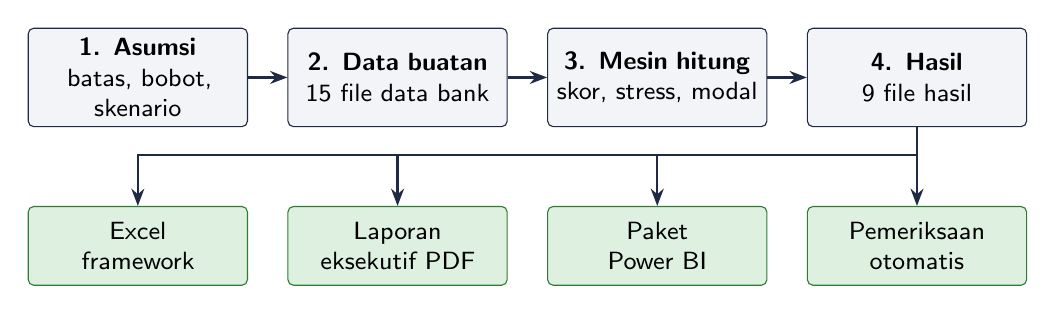
\begin{tikzpicture}[node distance=0.55cm and 0.5cm,
  box/.style={draw=navy,fill=softgrey,rounded corners=2pt,align=center,minimum height=1.25cm,text width=2.55cm,font=\small},
  outbox/.style={draw=ermgreen,fill=tintgreen!60,rounded corners=2pt,align=center,minimum height=1.0cm,text width=2.55cm,font=\small},
  arr/.style={-{Stealth[length=2.2mm]},thick,navy}]
\node[box] (cfg) {\textbf{1. Asumsi}\\batas, bobot, skenario};
\node[box,right=of cfg] (gen) {\textbf{2. Data buatan}\\15 file data bank};
\node[box,right=of gen] (eng) {\textbf{3. Mesin hitung}\\skor, stress, modal};
\node[box,right=of eng] (res) {\textbf{4. Hasil}\\9 file hasil};
\draw[arr] (cfg) -- (gen); \draw[arr] (gen) -- (eng); \draw[arr] (eng) -- (res);
\node[outbox,below=1.0cm of cfg] (xl) {Excel\\framework};
\node[outbox,right=of xl] (pdf) {Laporan\\eksekutif PDF};
\node[outbox,right=of pdf] (pbi) {Paket\\Power BI};
\node[outbox,right=of pbi] (tst) {Pemeriksaan\\otomatis};
\draw[arr] (res.south) -- ++(0,-0.35) -| (xl.north);
\draw[arr] (res.south) -- ++(0,-0.35) -| (pdf.north);
\draw[arr] (res.south) -- ++(0,-0.35) -| (pbi.north);
\draw[arr] (res.south) -- (tst.north);
\end{tikzpicture}
\caption{Dari asumsi sampai laporan. Semua angka di laporan dan Excel berasal dari file hasil (langkah 4).}
\end{figure}

\subsection{Hasil utama posisi September 2026}
\begin{table}[H]
\centering
\begin{tabular}{lccc}
\toprule
 & \textbf{Baseline} & \textbf{Adverse} & \textbf{Severe}\\
 & (kondisi normal) & (ekonomi melemah) & (krisis berat)\\
\midrule
Skor risiko enterprise (1--5) & 3{,}0 Moderate & 3{,}4 Moderate & 4{,}0 Moderate to High\\
Pemakaian limit rata-rata & 68\% & 78\% & 93\%\\
Indikator skor $\geq 4$ / skor 5 & 9 / 0 & 14 / 6 & 21 / 14\\
Rasio modal (KPMM) & 17{,}5\% & 15{,}8\% & 13{,}1\%\\
\bottomrule
\end{tabular}
\caption{Ringkasan hasil. Skor 1 berarti risiko sangat rendah, skor 5 berarti sangat tinggi.}
\end{table}

Cara membacanya: pada kondisi normal, profil risiko ASB berada di level \textbf{Moderate}. Risiko tertinggi adalah Compliance (3{,}6), Operational (3{,}6), Strategic (3{,}3). Pada skenario krisis berat, skor enterprise naik menjadi 4{,}0 dan rasio modal turun dari 17{,}5\% menjadi 13{,}1\%. Modal masih di atas batas minimum project (10{,}5\%).

\section{Isi File ZIP}\label{sec:zip}

Setelah file ZIP diekstrak, Anda akan mendapat satu folder utama:

\begin{center}\file{enterprise-risk-management}\end{center}

Isinya dikelompokkan seperti rak arsip:

\begin{longtable}{>{\raggedright\arraybackslash}p{4.3cm}>{\raggedright\arraybackslash}p{10.6cm}}
\toprule
\textbf{Folder / file} & \textbf{Isi dan kegunaan}\\
\midrule
\endhead
\file{report/} & \textbf{Laporan eksekutif PDF} (9 halaman). File paling mudah untuk mulai. \\
\file{excel/} & \textbf{Excel framework} dengan 10 sheet: taksonomi risiko, batas, contoh hitung, hasil stress, tracker tindakan. \\
\file{regulatory/} & Pemetaan rujukan regulasi beserta status yang sudah diperiksa. \\
\file{dashboard/} & Bahan dashboard Power BI: 13 tabel data, daftar rumus DAX, dan spesifikasi tampilan per halaman. \\
\file{data/output/} & \textbf{9 file hasil hitung} (CSV). Semua angka laporan berasal dari sini. \\
\file{data/raw/} & \textbf{15 file data bank buatan} (CSV), sekitar 96.224 baris. \\
\file{data/reference/} & Dokumen spesifikasi, batas setiap indikator, bobot, skenario, register risiko baru, dan pustaka tindakan. Dianggap \emph{read-only}. \\
\file{config/} & Profil bank (neraca) dan koefisien stress testing, dalam format teks YAML yang bisa dibuka dengan Notepad. \\
\file{notebooks/} & Lima notebook Jupyter untuk eksplorasi dan grafik. \\
\file{src/erm/} & Kode program (mesin hitung). Tidak perlu dibuka untuk pemakaian biasa. \\
\file{tests/} & Pemeriksaan otomatis yang memastikan semua angka konsisten. \\
\file{docs/} & Panduan ini (file \file{.tex} dan \file{.pdf}). \\
\file{run\_\allowbreak{}all.py} & Satu perintah untuk menjalankan semua langkah (cocok untuk Windows). \\
\file{Makefile} & Perintah singkat untuk Mac/Linux (\file{make all}, \file{make report}, dan seterusnya). \\
\file{README.md} & Ringkasan teknis project. \\
\file{pyproject.toml} & Daftar paket Python yang dibutuhkan. \\
\bottomrule
\end{longtable}

\section{Cara Cepat: Melihat Hasil Tanpa Menjalankan Apa pun}\label{sec:quick}

Semua hasil sudah tersedia di dalam ZIP. Anda tidak wajib menginstal apa pun untuk melihatnya.

\begin{stepbox}{Langkah 1 --- Baca laporan eksekutif}
Buka \file{report/ERM\_\allowbreak{}Executive\_\allowbreak{}Report.pdf} dengan pembaca PDF biasa. Halaman 1 berisi ringkasan dan keputusan yang diminta dari Direksi. Penjelasan per halaman ada di Bagian \ref{sec:report}.
\end{stepbox}

\begin{stepbox}{Langkah 2 --- Buka Excel framework}
Buka \file{excel/ERM\_\allowbreak{}Framework.xlsx} dengan Microsoft Excel, LibreOffice Calc, atau Google Sheets. Mulai dari sheet \file{06\_\allowbreak{}Risk\_\allowbreak{}Assessment} untuk melihat profil risiko September 2026. Penjelasan per sheet ada di Bagian \ref{sec:excel}.
\end{stepbox}

\begin{stepbox}{Langkah 3 --- Lihat data hasil}
File di \file{data/output/} bisa dibuka di Excel (\emph{File $\rightarrow$ Open}, pilih file \file{.csv}). Isi setiap file dijelaskan di Bagian \ref{sec:csv}.
\end{stepbox}

\begin{warnbox}[Membuka CSV di Excel berbahasa Indonesia]
File CSV memakai \textbf{titik} sebagai pemisah desimal dan \textbf{koma} sebagai pemisah kolom. Jika Excel Anda memakai format Indonesia, angka bisa terbaca salah (misalnya 2.8 menjadi 28). Solusinya: gunakan \emph{Data $\rightarrow$ From Text/CSV}, lalu pilih \emph{Delimiter: Comma} dan \emph{Locale / File origin: English (United States)}.
\end{warnbox}
\section{Persiapan Komputer}\label{sec:persiapan}

Bagian ini hanya diperlukan jika Anda ingin \textbf{membuat ulang} data dan laporan, atau mencoba mengubah asumsi.

\subsection{Yang perlu dipasang}

\begin{center}
\begin{tabularx}{\linewidth}{>{\bfseries}p{3.4cm}>{\raggedright\arraybackslash}p{2.3cm}X}
\toprule
Program & Wajib? & Kegunaan \\
\midrule
Python 3.11 atau lebih baru & Wajib & Menjalankan mesin hitung. Unduh dari \url{https://www.python.org/downloads/}. \\
Paket Python & Wajib & pandas, numpy, pyyaml, openpyxl, matplotlib, reportlab, pdfplumber, pillow, pytest. Dipasang otomatis (langkah di bawah). \\
LibreOffice & Disarankan & Menghitung ulang rumus Excel saat file dibuat, agar pemeriksaan otomatis bisa membaca nilainya. Unduh dari \url{https://www.libreoffice.org}. \\
Microsoft Excel & Opsional & Membuka Excel framework. \\
Power BI Desktop & Opsional & Merakit dashboard (Windows). \\
Jupyter & Opsional & Membuka notebook. \\
\bottomrule
\end{tabularx}
\end{center}

\subsection{Langkah pemasangan}

\begin{stepbox}{1. Ekstrak ZIP}
Klik kanan \file{erm\_\allowbreak{}final.zip} $\rightarrow$ \emph{Extract All}. Simpan di lokasi yang mudah, misalnya \file{Documents}. Hindari folder yang namanya mengandung spasi aneh atau terlalu panjang.
\end{stepbox}

\begin{stepbox}{2. Pasang Python}
Saat memasang Python di Windows, \textbf{centang ``Add python.exe to PATH''} di layar pertama installer. Untuk memastikan Python terpasang, buka \emph{Command Prompt} (Windows) atau \emph{Terminal} (Mac), lalu ketik:
\begin{lstlisting}
python --version
\end{lstlisting}
Jika muncul \texttt{Python 3.11.x} atau lebih baru, lanjutkan. Di Mac, perintahnya bisa jadi \texttt{python3}.
\end{stepbox}

\begin{stepbox}{3. Masuk ke folder project}
Di Command Prompt atau Terminal, pindah ke folder hasil ekstrak. Contoh (sesuaikan lokasinya):
\begin{lstlisting}
cd Documents\enterprise-risk-management
\end{lstlisting}
Tips di Windows: buka folder tersebut di File Explorer, klik kolom alamat, ketik \texttt{cmd}, lalu tekan Enter. Command Prompt langsung terbuka di folder itu.
\end{stepbox}

\begin{stepbox}{4. Pasang paket yang dibutuhkan (sekali saja)}
\begin{lstlisting}
python -m pip install -e ".[dev]"
\end{lstlisting}
Tunggu sampai selesai, biasanya 1--5 menit tergantung koneksi internet.
\end{stepbox}

\begin{tipbox}[Tips: lingkungan terpisah (opsional)]
Agar paket project tidak bercampur dengan program Python lain, Anda bisa membuat lingkungan khusus sebelum langkah 4:
\begin{lstlisting}
python -m venv .venv
.venv\Scripts\activate        (Windows)
source .venv/bin/activate     (Mac/Linux)
\end{lstlisting}
Setiap kali membuka Command Prompt baru, jalankan lagi baris \texttt{activate} yang sesuai.
\end{tipbox}
\section{Menjalankan Project}\label{sec:jalankan}

\subsection{Cara paling mudah: satu perintah}

Dari dalam folder project, ketik:
\begin{lstlisting}
python run_all.py
\end{lstlisting}

Komputer akan menjalankan enam tahap berikut secara berurutan. Di komputer biasa, semuanya selesai dalam sekitar 30--90 detik.

\begin{center}
\begin{tabularx}{\linewidth}{>{\bfseries}p{1.1cm}>{\raggedright\arraybackslash}p{4.4cm}X}
\toprule
Tahap & Yang terjadi & Hasil \\
\midrule
1/5 & Membuat data bank buatan & 15 file di \file{data/raw/} \\
2/5 & Menghitung indikator, skor, stress, modal, dan tindakan & 9 file di \file{data/output/} \\
3/5 & Membuat Excel framework & \file{excel/ERM\_\allowbreak{}Framework.xlsx} dan \file{regulatory/Regulatory\_\allowbreak{}Mapping.xlsx} \\
4/5 & Membuat paket Power BI & 13 tabel di \file{dashboard/model/} \\
5/5 & Membuat laporan eksekutif & \file{report/ERM\_\allowbreak{}Executive\_\allowbreak{}Report.pdf} \\
Akhir & Pemeriksaan otomatis & Tulisan \texttt{100 passed} bila semua cocok \\
\bottomrule
\end{tabularx}
\end{center}

\begin{infobox}[Hasilnya selalu sama]
Data buatan memakai ``angka acak tetap'' (\emph{seed} 42). Setiap kali dijalankan ulang tanpa perubahan asumsi, hasilnya identik sampai angka terakhir. Ini memudahkan pengecekan dan membuat hasil bisa diulang siapa pun.
\end{infobox}

Jika hanya ingin membuat file tanpa menjalankan pemeriksaan (lebih cepat):
\begin{lstlisting}
python run_all.py --no-test
\end{lstlisting}

\subsection{Alternatif untuk Mac/Linux: perintah make}

Jika program \texttt{make} tersedia (umumnya ada di Mac dan Linux), perintah berikut setara:

\begin{center}
\begin{tabularx}{\linewidth}{>{\ttfamily}p{3.4cm}X}
\toprule
\textrm{\textbf{Perintah}} & \textbf{Fungsi} \\
\midrule
make all & Semua tahap, termasuk pemeriksaan \\
make data & Hanya membuat data buatan \\
make engine & Hanya menghitung hasil \\
make excel & Hanya membuat Excel (dan regulatory mapping) \\
make powerbi & Hanya membuat paket Power BI \\
make report & Excel + Power BI + laporan PDF \\
make test & Hanya menjalankan pemeriksaan \\
\bottomrule
\end{tabularx}
\end{center}

\subsection{Menjalankan per langkah tanpa make (Windows)}

\begin{lstlisting}
set PYTHONPATH=src
python -m erm.generator
python -m erm engine
python -m erm excel
python -m erm powerbi
python -m erm report
python -m pytest -q
\end{lstlisting}
Di Mac/Linux, ganti baris pertama dengan \texttt{export PYTHONPATH=src}.

\begin{warnbox}[Urutan penting]
Langkah harus dijalankan berurutan: data $\rightarrow$ hasil hitung $\rightarrow$ Excel/Power BI/laporan. Jika Anda mengubah data atau asumsi lalu hanya membuat laporan tanpa menghitung ulang, laporan akan memakai hasil lama dan pemeriksaan otomatis akan gagal.
\end{warnbox}

\subsection{Tanda berhasil}

Di akhir proses akan muncul baris seperti:
\begin{lstlisting}
100 passed in 12.3s
\end{lstlisting}
Artinya semua pemeriksaan lolos. Jika muncul kata \texttt{failed}, lihat Bagian \ref{sec:masalah}.
\section{Istilah Dasar yang Perlu Dipahami}\label{sec:istilah}

\subsection{KRI dan empat batasnya}

\textbf{KRI} (\emph{Key Risk Indicator}) adalah angka pemantau risiko, misalnya \emph{NPF gross}, jumlah insiden per bulan, atau rasio pembiayaan terhadap dana pihak ketiga (FDR). Project ini memakai \textbf{42 KRI} yang tersebar di 10 jenis risiko, ditambah satu indikator modal (CAP01, KPMM).

Setiap KRI punya empat batas (\emph{cut-point}). Contoh untuk NPF gross, yang makin rendah makin baik:

\begin{center}
\begin{tabular}{cccccc}
\toprule
\textbf{Nilai NPF} & $\leq$ 2{,}0\% & $\leq$ 2{,}5\% & $\leq$ 3{,}0\% & $\leq$ 3{,}5\% & $>$ 3{,}5\% \\
\midrule
\textbf{Skor} & 1 & 2 & 3 & 4 & 5 \\
\textbf{Nama batas} & c1 & c2 = \emph{appetite} & c3 = \emph{trigger} & c4 = \emph{limit} & --- \\
\bottomrule
\end{tabular}
\end{center}

Beberapa KRI justru makin tinggi makin baik, misalnya SLSI (indikator likuiditas) dan NIM. Untuk KRI seperti ini, urutan batasnya dibalik.

\subsection{Skor, zona, dan warna}

\begin{center}
\begin{tabularx}{\linewidth}{c>{\bfseries}p{3.2cm}Xc}
\toprule
Skor & Zona & Arti & Warna \\
\midrule
1 & Strong & Jauh di dalam batas aman & \tagG\\
2 & Within appetite & Masih dalam selera risiko & \tagG\\
3 & Watch & Di atas selera risiko, perlu diawasi & \tagA\\
4 & Tolerance breach & Melewati trigger, wajib tindakan 30 hari & \tagR\\
5 & Limit breach & Melewati limit, tindakan 14 hari dan eskalasi Direksi & \tagR\\
\bottomrule
\end{tabularx}
\end{center}

\subsection{Dari skor KRI menjadi skor risiko}

\begin{enumerate}
\item \textbf{Rata-rata tertimbang.} Skor KRI dalam satu jenis risiko dirata-rata dengan bobotnya. Contoh Credit: lima KRI dengan bobot 35\%, 15\%, 15\%, 15\%, 20\%.
\item \textbf{Aturan lantai (\emph{floor}).} Skor risiko tidak boleh lebih rendah dari skor KRI terburuk dikurangi 1,5. Tujuannya agar satu indikator yang sangat buruk tidak ``tertutupi'' oleh indikator lain yang baik.
\item \textbf{Penyesuaian judgment (\emph{override}).} Komite boleh menaikkan atau menurunkan skor maksimal 1,0 dengan alasan tertulis. Pada September 2026, Compliance dinaikkan dari 3{,}3 menjadi 3{,}6 karena ada potensi temuan pemeriksaan terkait akad yang belum sesuai opini DPS. Skor sebelum penyesuaian (\emph{model score}) selalu ditampilkan berdampingan dengan skor akhir (\emph{final score}).
\end{enumerate}

\subsection{Rating risiko}

\begin{center}
\begin{tabular}{llc}
\toprule
\textbf{Skor (dibulatkan 1 desimal)} & \textbf{Rating} & \textbf{Warna} \\
\midrule
kurang dari 1,5 & Low & \tagG \\
1,5 sampai kurang dari 2,5 & Low to Moderate & \tagG \\
2,5 sampai kurang dari 3,5 & Moderate & \tagA \\
3,5 sampai kurang dari 4,5 & Moderate to High & \tagR \\
4,5 atau lebih & High & \tagR \\
\bottomrule
\end{tabular}
\end{center}

\subsection{Skor enterprise}

Sepuluh skor risiko digabung dengan \textbf{bobot materialitas}. Credit berbobot paling besar (25\%) karena pembiayaan adalah aset terbesar bank. Ada dua pengaman:
\begin{itemize}
\item Skor enterprise tidak boleh lebih rendah dari skor risiko terburuk dikurangi 1,5.
\item Jika ada risiko berbobot minimal 10\% yang skornya 4,5 atau lebih, skor enterprise minimal 3,5.
\end{itemize}

\subsection{Istilah lain}

\begin{longtable}{>{\bfseries\raggedright\arraybackslash}p{3.8cm}>{\raggedright\arraybackslash}p{11.1cm}}
\toprule
Istilah & Arti sederhana \\
\midrule
\endhead
Limit utilization & Seberapa ``penuh'' pemakaian limit. 100\% berarti tepat di limit. Angka untuk enterprise adalah rata-rata tertimbang semua KRI. \\
Tolerance breach & KRI dengan skor 4 atau 5 (sudah melewati trigger). \\
Limit breach & KRI dengan skor 5 (sudah melewati limit). \\
Trend: Deteriorating / Improving / Stable & Membandingkan rata-rata 3 bulan terakhir dengan 3 bulan sebelumnya. Label ``Deteriorating'' berarti memburuk lebih dari 10\% rentang batasnya. Lima bulan pertama berlabel ``Insufficient history'' karena datanya belum cukup. \\
Early warning & KRI yang masih skor 1--3, tetapi jika garis trennya diteruskan akan melewati batas berikutnya dalam 3 bulan. \\
Emerging risk & Risiko baru yang belum punya KRI: siber, AI/model, dan iklim. \\
Stress testing & Simulasi dampak skenario ekonomi buruk terhadap KRI, skor, dan modal. \\
KPMM & Kewajiban Penyediaan Modal Minimum: modal dibagi Aset Tertimbang Menurut Risiko (ATMR). \\
SLSI & Indikator likuiditas buatan project (\emph{Synthetic Liquidity Stress Indicator}). \textbf{Bukan} LCR resmi. \\
Displaced commercial risk & Tekanan bagi bank syariah untuk mengorbankan bagi hasilnya agar deposan tidak pindah ke bank lain. \\
DPS & Dewan Pengawas Syariah. \\
\bottomrule
\end{longtable}
\section{Membaca Laporan Eksekutif (PDF)}\label{sec:report}

File \file{report/ERM\_\allowbreak{}Executive\_\allowbreak{}Report.pdf} terdiri dari 9 halaman dengan 10 bagian. Semua angka di laporan dibaca otomatis dari \file{data/output/}, tidak diketik manual. Setiap angka yang tercetak dicatat bersama sumbernya di \file{report/ERM\_\allowbreak{}Executive\_\allowbreak{}Report\_\allowbreak{}facts.json}.

\begin{longtable}{>{\bfseries}p{0.8cm}>{\raggedright\arraybackslash}p{3.8cm}>{\raggedright\arraybackslash}p{10.2cm}}
\toprule
Hal. & Bagian & Yang perlu diperhatikan \\
\midrule
\endhead
1 & Executive Summary & Lima kotak angka utama (skor enterprise 3{,}0, rating Moderate, pemakaian limit 68\%, breach 9/0, emerging risk 3), pesan kunci, dan keputusan yang diminta dari Direksi. \\
2 & Framework & Bobot tiap risiko, jumlah KRI, arti skor 1--5, dan cara skor digabung. \\
3 & Risk Profile & Tabel skor per risiko (weighted, floor, model, override, final) dan \emph{heatmap} 12 bulan. Warna sel mengikuti rating. Dua grafik kecil: tren skor enterprise dan jumlah breach. \\
4 & Risk Appetite Monitoring & Enam grafik KRI utama dengan garis appetite (hijau), trigger (kuning), dan limit (merah), serta tabel semua KRI yang skornya 4 atau lebih. \\
5 & Key Developments & Cerita perkembangan: kualitas pembiayaan, insiden digital, likuiditas, bagi hasil, komplain, dan kepatuhan syariah; plus daftar KRI memburuk dan early warning. \\
6 & Stress Testing \& Capital Overlay & Skenario makro, skor per skenario, grafik \emph{waterfall} (kontribusi tiap risiko), grafik kerugian, dan tabel KPMM. \\
7 & Interdependency \& Emerging Risks & Diagram jalur penularan antar risiko dan register risiko baru. \\
8 & Management Actions & Tracker tindakan: status Open (kuning), Overdue (merah), Closed (hijau). \\
9 & Methodology, Limitations \& Disclaimer & Cara kerja, batasan, dan disclaimer. \\
\bottomrule
\end{longtable}

\begin{tipbox}[Cara menjelaskan dalam 1 menit]
``Framework ini memantau 42 KRI di 10 jenis risiko bank syariah. Posisi September 2026 berada di level Moderate dengan 9 KRI melewati trigger, terutama likuiditas, operasional digital, dan pertumbuhan pembiayaan yang terlalu agresif. Dalam krisis berat skor naik ke 4{,}0 dan KPMM turun ke 13{,}1\%. Pendorong terbesar erosi modal justru penurunan nilai sukuk, bukan kredit.''
\end{tipbox}
\section{Menggunakan Excel Framework}\label{sec:excel}

File \file{excel/ERM\_\allowbreak{}Framework.xlsx} berisi 10 sheet. Sebagian angka berupa \textbf{rumus hidup}: jika sel input diubah, hasilnya ikut berubah.

\subsection{Kode warna sel}

\begin{center}
\begin{tabularx}{\linewidth}{>{\raggedright\arraybackslash}p{4.5cm}X}
\toprule
\textbf{Tampilan} & \textbf{Arti} \\
\midrule
{\color{inputblue}\textbf{Teks biru}} & Angka input atau hasil yang disalin dari mesin hitung. \\
{\color{linkgreen}\textbf{Teks hijau}} & Rumus yang mengambil angka dari sheet lain. \\
\textbf{Teks hitam} & Rumus hitung di sheet yang sama. \\
\colorbox{yellow}{Latar kuning} & Sel yang boleh Anda ubah untuk simulasi (misalnya override). \\
Latar hijau/kuning/merah muda & Zona atau rating. \\
\bottomrule
\end{tabularx}
\end{center}

\subsection{Isi setiap sheet}

\begin{longtable}{>{\ttfamily\small\raggedright\arraybackslash}p{4.4cm}>{\raggedright\arraybackslash}p{10.4cm}}
\toprule
\textrm{\textbf{Sheet}} & \textbf{Isi dan cara pakai} \\
\midrule
\endhead
01\_\allowbreak{}Risk\_\allowbreak{}Taxonomy & Definisi 10 risiko, pendorong utama, bobot, pemilik risiko, dan jumlah KRI (rumus). \\
02\_\allowbreak{}Risk\_\allowbreak{}Appetite\_\allowbreak{}Statement & Pernyataan selera risiko per jenis risiko dan KRI utamanya, dengan nilai dan skor September 2026 yang ditautkan otomatis. \\
03\_\allowbreak{}KRI\_\allowbreak{}Definitions & Rumus setiap KRI dalam bahasa biasa, sumber datanya, frekuensi, dan pemiliknya. \\
04\_\allowbreak{}Thresholds & Tabel batas c1--c4 dan bobot semua KRI. Ada daftar pilihan (\emph{dropdown}) untuk arah KRI, serta kolom cek urutan batas dan jumlah bobot. \\
05\_\allowbreak{}Scoring\_\allowbreak{}Methodology & Aturan skor, rating, dan \textbf{contoh hitung Credit langkah demi langkah} dengan rumus hidup, dari skor tiap KRI sampai rating akhir. \\
06\_\allowbreak{}Risk\_\allowbreak{}Assessment & \textbf{Sheet utama.} Bagian A: 43 indikator September 2026. Bagian B: skor 10 risiko dengan kolom override kuning. Bagian C: skor enterprise, rating, pemakaian limit, dan jumlah breach. Kolom ``selisih'' harus 0. \\
07\_\allowbreak{}Stress\_\allowbreak{}Scenarios & Skenario makro, aturan stress per KRI, hasil per skenario, \textbf{simulasi KPMM dengan rumus hidup}, waterfall, dan nilai KRI setelah stress. \\
08\_\allowbreak{}Management\_\allowbreak{}Actions & Ringkasan jumlah per status (rumus), tracker tindakan, dan register emerging risk. \\
09\_\allowbreak{}Regulatory\_\allowbreak{}Mapping & Rujukan regulasi beserta status yang diperiksa per 2026-09-17 dan sumbernya. \\
10\_\allowbreak{}Change\_\allowbreak{}Log & Riwayat keputusan dan perubahan (approver fiktif). \\
\bottomrule
\end{longtable}

\subsection{Latihan simulasi di Excel}

\begin{stepbox}{Simulasi 1 --- Mengubah judgment override}
\begin{enumerate}
\item Buka sheet \file{06\_\allowbreak{}Risk\_\allowbreak{}Assessment}, cari Bagian B.
\item Pada baris \emph{Compliance}, kolom \emph{override $\Delta$} (kuning), ubah \texttt{0,3} menjadi \texttt{0}.
\item Perhatikan skor final Compliance turun ke 3{,}3 dan ratingnya berubah menjadi Moderate. Skor enterprise di Bagian C ikut turun sedikit.
\item Kolom ``selisih formula -- engine'' tidak lagi 0 karena Anda menyimpang dari hasil resmi. Kembalikan ke \texttt{0,3} setelah selesai.
\end{enumerate}
Nilai override hanya boleh antara $-1$ dan $+1$; Excel akan menolak angka di luar rentang itu.
\end{stepbox}

\begin{stepbox}{Simulasi 2 --- Mengubah loss rate kredit}
\begin{enumerate}
\item Buka sheet \file{07\_\allowbreak{}Stress\_\allowbreak{}Scenarios}, cari Bagian D (parameter kuning).
\item Ubah \emph{Loss rate kredit} dari \texttt{0,45} menjadi \texttt{0,60}.
\item Lihat kerugian kredit, total kerugian, dan KPMM pada skenario severe ikut berubah.
\end{enumerate}
\end{stepbox}

\begin{warnbox}
Perubahan di Excel hanya simulasi dan \textbf{tidak} memengaruhi mesin hitung, laporan PDF, atau file CSV. Untuk mengubah asumsi secara resmi, ikuti Bagian \ref{sec:ubah}. Jika Anda menyimpan Excel yang sudah diubah lalu menjalankan pemeriksaan otomatis, sebagian pemeriksaan Excel akan gagal; buat ulang file dengan \texttt{python run\_\allowbreak{}all.py}.
\end{warnbox}

\begin{infobox}[Excel tidak menampilkan angka?]
Jika sel rumus tampak kosong, tekan \texttt{Ctrl+Alt+F9} (Windows) untuk memaksa Excel menghitung ulang. File sudah diatur agar dihitung ulang otomatis saat dibuka.
\end{infobox}
\section{Memahami File Hasil (data/output)}\label{sec:csv}

\begin{longtable}{>{\ttfamily\small\raggedright\arraybackslash}p{4.6cm}>{\raggedright\arraybackslash}p{4.9cm}>{\raggedright\arraybackslash}p{5.3cm}}
\toprule
\textrm{\textbf{File}} & \textbf{Isi} & \textbf{Kolom penting} \\
\midrule
\endhead
kri\_\allowbreak{}monthly.csv & Satu baris per bulan per indikator (12 $\times$ 43). & nilai, skor, zona, warna, pemakaian limit, trend, early warning \\
risk\_\allowbreak{}scores\_\allowbreak{}monthly.csv & Satu baris per bulan per jenis risiko (12 $\times$ 10). & weighted, floor, model, override, final, rating, warna \\
enterprise\_\allowbreak{}profile\_\allowbreak{}monthly.csv & Satu baris per bulan. & skor enterprise, rating, pemakaian limit, jumlah breach, emerging risk \\
stress\_\allowbreak{}results.csv & Nilai dan skor setiap indikator sebelum dan sesudah stress, per skenario. & base\_\allowbreak{}value, stressed\_\allowbreak{}value, base\_\allowbreak{}score, stressed\_\allowbreak{}score \\
stress\_\allowbreak{}risk\_\allowbreak{}scores.csv & Skor 10 risiko per skenario. & model, final, rating, kontribusi terhadap perubahan enterprise \\
stress\_\allowbreak{}enterprise\_\allowbreak{}summary.csv & Ringkasan enterprise per skenario. & skor, rating, pemakaian limit, jumlah breach \\
stress\_\allowbreak{}waterfall.csv & Data grafik waterfall baseline $\rightarrow$ adverse/severe. & driver, kontribusi, kumulatif \\
capital\_\allowbreak{}overlay.csv & Dampak skenario ke modal. & kerugian kredit, sukuk, operasional, DCR; modal; ATMR; KPMM; skor CAP01 \\
management\_\allowbreak{}actions.csv & Tracker tindakan otomatis. & temuan, tindakan, pemilik, jatuh tempo, status \\
\bottomrule
\end{longtable}

\begin{infobox}[Presisi angka]
Angka di file CSV disimpan lengkap (misalnya skor Liquidity 2{,}65). Laporan dan Excel menampilkannya dibulatkan 1 desimal (2{,}7). Rating selalu ditentukan dari skor yang sudah dibulatkan.
\end{infobox}

\subsection{Data bank buatan (data/raw)}

Data ini adalah ``bahan baku'' mesin hitung. Semuanya konsisten dengan neraca ASB: total aset Rp 60.000 miliar, pembiayaan Rp 41.000 miliar, DPK Rp 48.000 miliar, dan modal Rp 7.000 miliar pada September 2026. Semua nominal dalam Rp miliar.

\begin{longtable}{>{\ttfamily\small\raggedright\arraybackslash}p{4.8cm}r>{\raggedright\arraybackslash}p{7.6cm}}
\toprule
\textrm{\textbf{File}} & \textbf{Baris} & \textbf{Isi} \\
\midrule
\endhead
balance\_\allowbreak{}sheet\_\allowbreak{}monthly.csv & 210 & Neraca bulanan per pos (aset, liabilitas, ekuitas) \\
capital\_\allowbreak{}monthly.csv & 15 & Modal, ATMR, pendapatan, laba vs anggaran \\
financing\_\allowbreak{}portfolio.csv & 85.333 & Pembiayaan per nasabah per bulan (segmen, sektor, akad, kolektibilitas) \\
deposits\_\allowbreak{}monthly.csv & 45 & Saldo giro, tabungan, deposito dan tingkat bagi hasil \\
top\_\allowbreak{}depositors.csv & 300 & 20 deposan terbesar per bulan \\
maturity\_\allowbreak{}profile.csv & 60 & Aset dan liabilitas jatuh tempo per kelompok waktu \\
market\_\allowbreak{}positions.csv & 45 & Posisi valas (USD, SAR, SGD) \\
investment\_\allowbreak{}portfolio.csv & 375 & Kepemilikan sukuk (SBSN dan korporasi fiktif) \\
rate\_\allowbreak{}of\_\allowbreak{}return\_\allowbreak{}monthly.csv & 15 & Imbal hasil pembiayaan, ekspektasi vs realisasi deposan, NIM \\
operational\_\allowbreak{}events.csv & 321 & Log insiden operasional \\
compliance\_\allowbreak{}events.csv & 32 & Pelanggaran kepatuhan dan temuan DPS \\
legal\_\allowbreak{}cases.csv & 11 & Kasus hukum \\
complaints.csv & 9.417 & Komplain nasabah \\
sentiment\_\allowbreak{}monthly.csv & 30 & Sebutan media dan media sosial (total dan negatif) \\
strategic\_\allowbreak{}monthly.csv & 15 & Pertumbuhan pembiayaan, cost to income, inisiatif strategis \\
\bottomrule
\end{longtable}

\begin{infobox}[Mengapa data dimulai sebelum Oktober 2025?]
Beberapa indikator memerlukan data bulan-bulan sebelumnya, misalnya penurunan DPK dalam 3 bulan atau kerugian 12 bulan terakhir. Karena itu data bulanan dimulai Juli 2025 dan log kejadian dimulai Oktober 2024. Laporan hanya menampilkan Oktober 2025 -- September 2026.
\end{infobox}
\section{Stress Testing dan Dampak ke Modal}\label{sec:stress}

\subsection{Tiga skenario}

\begin{center}
\begin{tabular}{lrrr}
\toprule
\textbf{Asumsi makro} & \textbf{Baseline} & \textbf{Adverse} & \textbf{Severe}\\
\midrule
Pertumbuhan ekonomi (\%) & 5{,}0 & 2{,}0 & -1{,}0\\
Inflasi (\%) & 3{,}0 & 4{,}5 & 6{,}0\\
Kenaikan suku bunga acuan (bps) & 0{,}0 & 100{,}0 & 250{,}0\\
Pelemahan rupiah (\%) & 0{,}0 & 10{,}0 & 25{,}0\\
Penurunan DPK 3 bulan (\%) & 0{,}0 & 5{,}0 & 12{,}0\\
Penurunan harga sukuk (\%) & 0{,}0 & -5{,}0 & -15{,}0\\
Tambahan insiden operasional (\%) & 0{,}0 & 20{,}0 & 50{,}0\\
Tambahan pertumbuhan komplain (poin) & 0{,}0 & 30{,}0 & 60{,}0\\
Kenaikan ATMR (\%) & 0{,}0 & 2{,}0 & 5{,}0\\
\bottomrule
\end{tabular}
\end{center}

Setiap skenario diterapkan ke nilai KRI September 2026 memakai aturan sederhana yang tertulis di \file{config/stress\_\allowbreak{}parameters.yaml}. Contohnya: NPF naik 0,20 poin untuk setiap 1 poin penurunan pertumbuhan ekonomi. Setelah itu skor dihitung ulang dengan aturan yang persis sama seperti pemantauan bulanan. Neraca dianggap tidak berubah dan belum ada tindakan manajemen, sehingga hasilnya adalah dampak kotor (\emph{gross impact}).

\subsection{Hasil skor per skenario}

\begin{center}
\begin{tabular}{lccc}
\toprule
\textbf{Risiko} & \textbf{Baseline} & \textbf{Adverse} & \textbf{Severe}\\
\midrule
Credit & \cellcolor{tintamber}3{,}0 & \cellcolor{tintred}3{,}5 & \cellcolor{tintred}4{,}0\\
Market & \cellcolor{tintgreen}2{,}3 & \cellcolor{tintred}3{,}5 & \cellcolor{tintred}3{,}5\\
Liquidity & \cellcolor{tintamber}2{,}7 & \cellcolor{tintamber}3{,}0 & \cellcolor{tintred}4{,}5\\
Operational & \cellcolor{tintred}3{,}6 & \cellcolor{tintred}3{,}8 & \cellcolor{tintred}4{,}5\\
Strategic & \cellcolor{tintamber}3{,}3 & \cellcolor{tintred}3{,}5 & \cellcolor{tintred}4{,}1\\
Compliance & \cellcolor{tintred}3{,}6 & \cellcolor{tintred}3{,}6 & \cellcolor{tintred}3{,}6\\
Legal & \cellcolor{tintgreen}2{,}2 & \cellcolor{tintgreen}2{,}2 & \cellcolor{tintgreen}2{,}2\\
Reputation & \cellcolor{tintamber}2{,}6 & \cellcolor{tintred}3{,}5 & \cellcolor{tintred}3{,}5\\
Rate of Return & \cellcolor{tintamber}3{,}1 & \cellcolor{tintred}3{,}7 & \cellcolor{tintred}4{,}2\\
Investment & \cellcolor{tintgreen}2{,}2 & \cellcolor{tintamber}3{,}0 & \cellcolor{tintred}3{,}5\\
\midrule
\textbf{Enterprise} & \cellcolor{tintamber}\textbf{3{,}0} & \cellcolor{tintamber}\textbf{3{,}4} & \cellcolor{tintred}\textbf{4{,}0}\\
\bottomrule
\end{tabular}
\end{center}

\subsection{Waterfall: risiko mana yang paling mendorong kenaikan?}

Kontribusi dihitung sebagai kenaikan skor risiko dikalikan bobotnya. Dari baseline ke severe:

\begin{center}
\begin{tabular}{lr}
\toprule
\textbf{Pendorong} & \textbf{Kontribusi}\\
\midrule
Liquidity & +0{,}27\\
Credit & +0{,}25\\
Rate of Return & +0{,}11\\
Operational & +0{,}10\\
Investment & +0{,}09\\
Strategic & +0{,}06\\
Market & +0{,}06\\
Reputation & +0{,}05\\
\midrule
\textbf{Total kenaikan skor enterprise} & \textbf{+1{,}00}\\
\bottomrule
\end{tabular}
\end{center}

\subsection{Capital Adequacy Overlay (KPMM)}

\begin{center}
\begin{tabular}{lrrr}
\toprule
\textbf{Rp miliar} & \textbf{Baseline} & \textbf{Adverse} & \textbf{Severe}\\
\midrule
Kerugian kredit & -- & 129 & 268\\
Penurunan nilai sukuk & -- & 300 & 900\\
Kerugian operasional & -- & 18 & 45\\
Biaya menjaga bagi hasil deposan (DCR) & -- & 120 & 300\\
\textbf{Total kerugian} & -- & 567 & 1.513\\
Modal setelah stress & 7.000 & 6.433 & 5.487\\
ATMR setelah stress & 40.000 & 40.800 & 42.000\\
\midrule
\textbf{KPMM} & \textbf{17{,}5\%} & \textbf{15{,}8\%} & \textbf{13{,}1\%}\\
\bottomrule
\end{tabular}
\end{center}

\begin{tipbox}[Pesan utama]
Pada skenario severe, penurunan nilai sukuk menyumbang sekitar 60\% dari total kerugian, lebih besar dari kerugian kredit. Ini menunjukkan risiko pasar dan investasi sama pentingnya dengan risiko kredit bagi bank syariah yang memegang banyak sukuk.
\end{tipbox}

\begin{infobox}[Jalur penularan antar risiko]
Diagram di laporan (halaman 7) menunjukkan, misalnya, bahwa kenaikan suku bunga acuan menurunkan nilai sukuk (Market), memperlebar selisih bagi hasil (Rate of Return), dan mendorong deposan pindah bank (Liquidity). Jalur ini tercatat di \file{data/reference/interdependency\_\allowbreak{}edges.csv}.
\end{infobox}
\section{Management Actions dan Emerging Risk}\label{sec:actions}

\subsection{Tindakan otomatis}

Setiap KRI yang skornya mencapai 4 otomatis menghasilkan satu rencana tindakan dengan tenggat \textbf{30 hari}. Jika mencapai skor 5, tenggatnya \textbf{14 hari} dan wajib dieskalasi ke Direksi/Komite. Teks tindakan diambil dari \file{data/reference/action\_\allowbreak{}library.csv} dan tidak dikarang bebas. Tindakan dibuat sekali saat KRI pertama kali melewati batas, bukan setiap bulan.

\begin{center}
\begin{tabular}{lcl}
\toprule
\textbf{Status} & \textbf{Jumlah} & \textbf{Arti} \\
\midrule
Open & 5 & Masih berjalan dan belum lewat tenggat \\
Overdue & 4 & Masih berjalan dan sudah lewat tenggat per 30 September 2026 \\
Closed & 1 & KRI sudah kembali di bawah skor 4 \\
Superseded & 0 & Digantikan tindakan eskalasi karena KRI naik ke skor 5 \\
\bottomrule
\end{tabular}
\end{center}

KRI yang melewati trigger pada September 2026:
\begin{itemize}
\item \textbf{CP02} Pelanggaran high-severity melewati target remediasi --- nilai 3{,}00, pemakaian limit 100\%
\item \textbf{CR02} NPF segmen UMKM --- nilai 5{,}30, pemakaian limit 88\%
\item \textbf{ST01} Deviasi pertumbuhan pembiayaan YoY vs target (absolut) --- nilai 7{,}00, pemakaian limit 88\%
\item \textbf{RR02} Gap return ekspektasi vs realisasi deposan --- nilai 0{,}70, pemakaian limit 87\%
\item \textbf{LQ04} Negative maturity gap $\leq$1 bulan (absolut) --- nilai 10{,}50, pemakaian limit 84\%
\item \textbf{OR01} Jumlah insiden operasional --- nilai 21{,}00, pemakaian limit 84\%
\item \textbf{RP01} Pertumbuhan volume komplain MoM --- nilai 25{,}03, pemakaian limit 83\%
\item \textbf{OR04} Repeat incident rate --- nilai 8{,}06, pemakaian limit 81\%
\item \textbf{OR03} Kerugian operasional rolling 12 bulan --- nilai 1{,}60, pemakaian limit 80\%
\end{itemize}

\subsection{Early warning}

KRI yang belum melewati trigger tetapi diperkirakan mendekati batas berikutnya: \textbf{CP04} (Temuan DPS (kepatuhan syariah) terbuka >90 hari), \textbf{LG04} (Kasus aging >365 hari), \textbf{LQ01} (Synthetic Liquidity Stress Indicator (SLSI)), \textbf{LQ05} (Penurunan DPK 3 bulan), \textbf{OR02} (Insiden high-severity (rolling 3 bulan)), \textbf{RR01} (Gap bagi hasil deposito vs benchmark pasar (benchmark - ASB)).

\subsection{Emerging risk register}

\begin{center}
\begin{tabularx}{\linewidth}{l>{\raggedright\arraybackslash}p{2.6cm}ccccX}
\toprule
\textbf{ID} & \textbf{Risiko} & \textbf{L} & \textbf{I} & \textbf{V} & \textbf{Prioritas} & \textbf{Status} \\
\midrule
ER01 & Cyber risk & 4 & 5 & 5 & 20{,}0 & Watch\\
ER02 & AI / model risk & 3 & 4 & 4 & 9{,}6 & Watch\\
ER03 & Climate risk & 3 & 4 & 2 & 4{,}8 & Monitor\\
\bottomrule
\end{tabularx}
\end{center}
L = kemungkinan, I = dampak, V = kecepatan (masing-masing 1--5). Prioritas = L $\times$ I $\times$ (V/5).
\section{Merakit Dashboard Power BI}\label{sec:powerbi}

Project \textbf{tidak} menyertakan file \file{.pbix} yang siap pakai. Yang disediakan adalah bahan lengkap untuk merakitnya sendiri di Power BI Desktop.

\begin{stepbox}{Langkah perakitan}
\begin{enumerate}
\item Buka Power BI Desktop $\rightarrow$ \emph{Get Data} $\rightarrow$ \emph{Text/CSV}.
\item Impor ke-13 file di \file{dashboard/model/}. Pada jendela impor, pilih \emph{File origin: 65001 UTF-8} dan \emph{Delimiter: Comma}. Klik \emph{Transform Data}, lalu set \emph{Locale} ke \emph{English (United States)} agar desimal terbaca benar.
\item Buka \emph{Model view}, lalu sambungkan tabel berawalan \file{fact\_\allowbreak{}} ke tabel berawalan \file{dim\_\allowbreak{}} melalui kolom kunci yang sama namanya (\file{date\_\allowbreak{}key}, \file{risk\_\allowbreak{}key}, \file{kri\_\allowbreak{}key}, \file{scenario\_\allowbreak{}key}, \file{bu\_\allowbreak{}key}). Daftar relasi lengkap ada di \file{dashboard/powerbi\_\allowbreak{}spec.md}.
\item Buat tabel kosong bernama \file{\_\allowbreak{}Measures} (\emph{Enter Data} $\rightarrow$ OK), lalu tempel setiap rumus dari \file{dashboard/DAX\_\allowbreak{}measures.md} sebagai \emph{New measure}.
\item Susun 6 halaman sesuai spesifikasi: Enterprise Overview, Risk Appetite, Risk Trend \& Early Warning, Enterprise Stress, Interdependency, Management Action.
\item Terapkan warna: hijau \texttt{\#2E7D32}, kuning \texttt{\#F9A825}, merah \texttt{\#C62828}.
\end{enumerate}
\end{stepbox}

\begin{infobox}[Konvensi skenario]
Tabel skor memuat dua jenis data: pemantauan bulanan dengan skenario \texttt{Actual}, dan hasil stress (Baseline, Adverse, Severe) yang ditempatkan pada tanggal September 2026. Gunakan slicer skenario untuk berpindah; jika slicer tidak dipilih, rumus memakai \texttt{Actual}.
\end{infobox}

\begin{tipbox}[Cek hasil rakitan]
Kartu skor enterprise September 2026 harus menunjukkan 3{,}0, pemakaian limit 68\%, dan breach 9/0. Jika berbeda, periksa pengaturan locale saat impor.
\end{tipbox}

\section{Notebook Jupyter}\label{sec:notebook}

Folder \file{notebooks/} berisi lima notebook untuk eksplorasi. Notebook tidak menyimpan logika sendiri; semuanya memanggil fungsi yang sama dengan mesin hitung.

\begin{center}
\begin{tabularx}{\linewidth}{>{\ttfamily\small}p{5.2cm}X}
\toprule
\textrm{\textbf{Notebook}} & \textbf{Isi} \\
\midrule
01\_\allowbreak{}data\_\allowbreak{}generation & Rekonsiliasi neraca dan data rinci \\
02\_\allowbreak{}kri\_\allowbreak{}risk\_\allowbreak{}appetite & Profil risiko dan KRI yang melewati trigger \\
03\_\allowbreak{}trend\_\allowbreak{}early\_\allowbreak{}warning & Grafik skor 12 bulan, KRI memburuk, dan early warning \\
04\_\allowbreak{}stress\_\allowbreak{}capital & Hasil stress, waterfall, dan grafik kerugian \\
05\_\allowbreak{}reporting & Membuat ulang deliverable dan tracker tindakan \\
\bottomrule
\end{tabularx}
\end{center}

Cara membuka: pasang Jupyter (\texttt{python -m pip install notebook}), jalankan \texttt{jupyter notebook} dari folder project, buka file di folder \file{notebooks}, lalu pilih \emph{Run All}. Notebook disimpan tanpa hasil, jadi tabel dan grafik baru muncul setelah dijalankan.
\section{Mencoba Mengubah Asumsi}\label{sec:ubah}

Project dirancang agar asumsi bisa diubah \textbf{tanpa menyentuh kode program}. Setelah mengubah, jalankan ulang \texttt{python run\_\allowbreak{}all.py --no-test}, lalu buka laporan dan Excel yang baru.

\begin{warnbox}[Sebelum mulai]
\begin{enumerate}
\item \textbf{Salin dulu seluruh folder project} (misalnya menjadi \file{erm-eksperimen}) dan bekerja di salinan itu. Versi asli tetap aman sebagai acuan.
\item Pemeriksaan otomatis dirancang untuk memastikan hasil \textbf{sama dengan spesifikasi asli}. Setelah asumsi diubah, sebagian pemeriksaan \textbf{pasti gagal}. Itu normal dan justru menandakan hasil Anda berbeda dari versi resmi.
\end{enumerate}
\end{warnbox}

\subsection{Mengubah koefisien stress testing}

Buka \file{config/stress\_\allowbreak{}parameters.yaml} dengan Notepad atau TextEdit. Contoh:
\begin{lstlisting}
CR01: {rule: additive, gdp_coef: 0.20, bps_coef: 0.10}
\end{lstlisting}
Ubah \texttt{gdp\_\allowbreak{}coef: 0.20} menjadi \texttt{0.30} agar NPF lebih sensitif terhadap perlambatan ekonomi. Di bagian \texttt{capital\_\allowbreak{}overlay}, Anda juga bisa mengubah \texttt{loss\_\allowbreak{}rate: 0.45}.

\begin{warnbox}[Aturan penulisan YAML]
Gunakan \textbf{titik} untuk desimal (\texttt{0.30}, bukan \texttt{0,30}), jangan ubah jumlah spasi di awal baris, dan jangan hapus titik dua. Kesalahan kecil membuat program berhenti dengan pesan error.
\end{warnbox}

\subsection{Mengubah skenario makro}

Buka \file{data/reference/macro\_\allowbreak{}scenarios.csv} di Excel atau Notepad. Ubah angka pada kolom \texttt{adverse} atau \texttt{severe}, misalnya kenaikan suku bunga severe dari 250 menjadi 300 bps. Simpan tetap sebagai CSV (koma sebagai pemisah).

\subsection{Mengubah batas atau bobot KRI}

Buka \file{data/reference/risk\_\allowbreak{}appetite.csv}. Kolom \texttt{c1}--\texttt{c4} adalah batas, dan \texttt{kri\_\allowbreak{}weight} adalah bobot.
\begin{itemize}
\item Bobot KRI dalam satu jenis risiko harus berjumlah 1,00.
\item Untuk KRI ``lower'' urutan batas harus naik (c1 $<$ c2 $<$ c3 $<$ c4); untuk ``higher'' harus turun.
\item Data buatan dikalibrasi terhadap kolom \texttt{value\_\allowbreak{}start\_\allowbreak{}2025\_\allowbreak{}10} dan \texttt{value\_\allowbreak{}target\_\allowbreak{}2026\_\allowbreak{}09}. Mengubah kolom ini akan mengubah data yang dihasilkan.
\end{itemize}

\subsection{Mengubah judgment override}

Buka \file{data/reference/judgment\_\allowbreak{}overrides.csv}. Selisih \texttt{final\_\allowbreak{}score} dan \texttt{model\_\allowbreak{}score} adalah besaran penyesuaian (maksimal $\pm$1,0). Kolom \texttt{period} dan \texttt{valid\_\allowbreak{}until} menentukan bulan berlakunya.

\subsection{Mengubah profil bank}

\file{config/bank\_\allowbreak{}profile.yaml} memuat neraca September 2026, modal, dan parameter likuiditas. Semua data buatan menyesuaikan diri dengan neraca ini. Perubahan besar (misalnya total aset) dapat membuat kalibrasi gagal, jadi lakukan perubahan kecil dan bertahap.

\begin{infobox}[Kembali ke versi asli]
Cara paling aman adalah mengekstrak ulang \file{erm\_\allowbreak{}final.zip}. File \file{data/reference/CHECKSUMS.sha256} menyimpan ``sidik jari'' file referensi asli; pemeriksaan otomatis memakainya untuk mendeteksi perubahan.
\end{infobox}
\section{Pemeriksaan Otomatis}\label{sec:test}

Perintah \texttt{python -m pytest -q} (atau tahap terakhir \texttt{run\_\allowbreak{}all.py}) menjalankan 100 pemeriksaan. Anda tidak perlu memahami kodenya; cukup lihat baris terakhir.

\begin{longtable}{>{\raggedright\arraybackslash}p{4.3cm}>{\raggedright\arraybackslash}p{10.5cm}}
\toprule
\textbf{Kelompok} & \textbf{Yang dipastikan} \\
\midrule
\endhead
Referensi & File acuan tidak berubah; bobot berjumlah 1,00; semua KRI dan koefisien sesuai spesifikasi. \\
Data buatan & Neraca seimbang setiap bulan; total data rinci sama dengan neraca; hasil identik bila dijalankan dua kali; alur cerita (NPF naik, insiden digital, DPK turun, komplain melonjak) terbukti. \\
Skor & Skor September 2026 sama dengan target; tren dan early warning sesuai; profil risiko identik dengan ringkasan spesifikasi. \\
Stress & Skor, rating, breach, pemakaian limit, dan KPMM tiga skenario sama dengan perhitungan acuan; skor tidak turun saat skenario makin berat; tidak ada model di luar cakupan. \\
Deliverable & Angka Excel dan laporan PDF sama dengan file hasil; paket Power BI lengkap dan relasinya konsisten. \\
Penutup & Struktur folder lengkap, notebook bisa dijalankan, regulatory mapping sudah berstatus terverifikasi. \\
\bottomrule
\end{longtable}

\textbf{Cara membaca hasil:}
\begin{itemize}
\item \texttt{100 passed} --- semua lolos.
\item \texttt{3 failed, 97 passed} --- ada 3 yang gagal. Di atas ringkasan akan tercetak nama pemeriksaan yang gagal, misalnya \texttt{test\_\allowbreak{}regression\_\allowbreak{}capital\_\allowbreak{}overlay}, beserta nilai yang diharapkan dan nilai yang didapat.
\end{itemize}
\section{Rujukan Regulasi}\label{sec:regulasi}

Pemetaan regulasi hanya menjelaskan \textbf{area yang menginspirasi} framework. Tidak ada klaim bahwa batas project sama dengan ketentuan. Status di bawah diperiksa per 2026-09-17 dari JDIH BPK dan laman regulasi OJK.

\begin{longtable}{>{\raggedright\arraybackslash}p{3.6cm}>{\raggedright\arraybackslash}p{5.2cm}>{\raggedright\arraybackslash}p{5.9cm}}
\toprule
\textbf{Area} & \textbf{Rujukan} & \textbf{Status} \\
\midrule
\endhead
Manajemen risiko BUS/UUS (10 jenis risiko) & POJK 65/POJK.03/2016 & \textbf{Berlaku} \\
Penilaian tingkat kesehatan BUS/UUS (RBBR) & POJK 8/POJK.03/2014 dan SEOJK 10/SEOJK.03/2014 & \textbf{Berlaku (POJK); SEOJK masih tercantum di laman OJK} \\
KPMM BUS & POJK 21/POJK.03/2014 & \textbf{Berlaku; perubahan tidak ditemukan} \\
Tata kelola syariah / DPS & POJK 2 Tahun 2024 (tata kelola syariah BUS/UUS); melengkapi POJK 17 Tahun 2023 (tata kelola bank umum) & \textbf{Berlaku} \\
Likuiditas (LCR/NSFR) BUS/UUS & POJK 20 Tahun 2025 & \textbf{Berlaku (pemenuhan bertahap)} \\
Posisi Devisa Neto (PDN) & PBI 5/13/PBI/2003 sebagaimana diubah terakhir dengan PBI 12/10/PBI/2010 & \textbf{Belum terkonfirmasi} \\
\bottomrule
\end{longtable}

\begin{warnbox}
Status peraturan bisa berubah setelah tanggal pemeriksaan, dan database JDIH dapat terlambat memperbarui catatan. Konfirmasi ulang ke JDIH OJK sebelum mengutipnya. Rincian dasar verifikasi dan tautan sumber ada di \file{regulatory/Regulatory\_\allowbreak{}Mapping.xlsx}. Panduan ini bukan pendapat hukum.
\end{warnbox}
\section{Batasan Project}\label{sec:batasan}

\begin{itemize}
\item \textbf{Sengaja tidak dibuat:} model PD/LGD/EAD, ECL/CKPN (PSAK 71), VaR dan Monte Carlo, ekonometrika, machine learning, perhitungan LCR/NSFR resmi, serta model distribusi bagi hasil.
\item \textbf{Stress statis:} neraca tidak bereaksi terhadap skenario dan belum ada tindakan manajemen. Indikator non-makro (konsentrasi, kepatuhan, hukum, sebagian reputasi) dianggap tidak berubah.
\item \textbf{Asumsi tidak dikalibrasi ke data historis:} loss rate kredit 45\%, koefisien stress, bobot, dan batas adalah pilihan analitis project.
\item \textbf{Data buatan:} beberapa indikator berbasis hitungan kecil (misalnya jumlah kasus) hanya mendekati nilai awal yang ditargetkan.
\item \textbf{SLSI bukan LCR.} Sejak POJK 20 Tahun 2025, BUS wajib memenuhi LCR dan NSFR secara bertahap (LCR minimum 80\% mulai Juni 2026). Project tidak menghitung rasio resmi tersebut.
\item \textbf{Rating} terinspirasi skala penilaian risiko perbankan Indonesia, tetapi bukan replika metodologi penilaian tingkat kesehatan bank.
\item \textbf{Power BI:} file \file{.pbix} harus dirakit manual.
\end{itemize}

\begin{tcolorbox}[colback=softgrey,colframe=navy,boxrule=0.6pt,arc=2pt,title=Disclaimer,fonttitle=\bfseries]
This project uses a fictional Islamic bank and fully synthetic data. All risk appetite thresholds, scenarios, sensitivities, and scoring rules are project-specific analytical assumptions created for educational and portfolio purposes. They do not represent any actual bank's internal limits, regulatory thresholds, or an official OJK risk profile rating.
\end{tcolorbox}
\section{Pemecahan Masalah}\label{sec:masalah}

\begin{longtable}{>{\raggedright\arraybackslash}p{5.6cm}>{\raggedright\arraybackslash}p{9.2cm}}
\toprule
\textbf{Masalah / pesan} & \textbf{Penyebab dan solusi} \\
\midrule
\endhead
\texttt{'python' is not recognized} atau \texttt{command not found} & Python belum terpasang atau belum masuk PATH. Pasang ulang Python dan centang \emph{Add python.exe to PATH}. Di Mac, coba \texttt{python3}. \\
\addlinespace[2pt]
\texttt{ModuleNotFoundError: No module named 'pandas'} (atau paket lain) & Paket belum dipasang. Jalankan \texttt{python -m pip install -e ".[dev]"} dari folder project. Jika memakai \texttt{.venv}, pastikan sudah diaktifkan. \\
\addlinespace[2pt]
\texttt{No module named 'erm'} & Perintah dijalankan dari folder yang salah, atau \texttt{PYTHONPATH} belum diatur. Pindah ke folder \file{enterprise-risk-management}, lalu gunakan \texttt{python run\_\allowbreak{}all.py}. \\
\addlinespace[2pt]
\texttt{'make' is not recognized} & Program make umumnya tidak ada di Windows. Gunakan \texttt{python run\_\allowbreak{}all.py}. \\
\addlinespace[2pt]
Tahap Excel menampilkan \texttt{status: skipped} & LibreOffice tidak ditemukan. File Excel tetap dibuat dan angkanya dihitung saat dibuka di Excel, tetapi pemeriksaan otomatis untuk Excel akan gagal. Pasang LibreOffice lalu jalankan ulang. \\
\addlinespace[2pt]
Pemeriksaan Excel gagal dengan pesan nilai \texttt{None} & Rumus Excel belum dihitung ulang (lihat baris sebelumnya), atau file Excel pernah disimpan setelah diubah manual. Jalankan ulang \texttt{python run\_\allowbreak{}all.py}. \\
\addlinespace[2pt]
\texttt{PermissionError} saat membuat Excel atau PDF & File sedang terbuka di Excel atau pembaca PDF. Tutup file tersebut lalu jalankan ulang. \\
\addlinespace[2pt]
Angka CSV di Excel terlihat aneh (misalnya 28 bukan 2.8) & Pengaturan desimal Indonesia. Impor lewat \emph{Data $\rightarrow$ From Text/CSV} dengan locale English (United States). \\
\addlinespace[2pt]
Setelah mengubah asumsi, banyak pemeriksaan gagal & Normal. Pemeriksaan membandingkan hasil dengan spesifikasi asli. Gunakan \texttt{run\_\allowbreak{}all.py --no-test} untuk eksperimen. \\
\addlinespace[2pt]
\texttt{kalibrasi neraca menghasilkan ... non-positif} atau \texttt{raking tidak konvergen} & Perubahan profil bank atau target KRI terlalu ekstrem sehingga data tidak bisa dibentuk. Kembalikan sebagian perubahan atau lakukan secara bertahap. \\
\addlinespace[2pt]
Error YAML (\texttt{ScannerError}, \texttt{ParserError}) & Ada salah ketik di file \file{.yaml}: spasi awal baris, titik dua, atau koma desimal. Bandingkan dengan salinan asli. \\
\addlinespace[2pt]
Proses sangat lambat atau berhenti di tahap Excel & LibreOffice sedang terbuka di latar belakang. Tutup semua jendela LibreOffice lalu ulangi. \\
\addlinespace[2pt]
\bottomrule
\end{longtable}
\appendix
\section{Lampiran: Daftar KRI dan Batasnya}\label{sec:lampiran-kri}

Arah \textbf{L} = makin rendah makin baik; \textbf{H} = makin tinggi makin baik. Kolom ``Sep-26'' adalah nilai hasil hitung dan skornya.

{\small
\begin{longtable}{@{}l>{\raggedright\arraybackslash}p{4.6cm}>{\raggedright\arraybackslash}p{1.7cm}cr>{\raggedright\arraybackslash}p{2.5cm}rc@{}}
\toprule
\textbf{ID} & \textbf{Nama KRI} & \textbf{Satuan} & \textbf{Arah} & \textbf{Bobot} & \textbf{c1 / c2 / c3 / c4} & \textbf{Sep-26} & \textbf{Skor}\\
\midrule
\endhead
\multicolumn{8}{l}{\cellcolor{softgrey}\textbf{Credit}}\\
CR01 & NPF gross & \% & L & 0{,}35 & 2 / 2{,}5 / 3 / 3{,}5 & 2{,}80 & \cellcolor{tintamber}3\\
CR02 & NPF segmen UMKM & \% & L & 0{,}15 & 3 / 4 / 5 / 6 & 5{,}30 & \cellcolor{tintred}4\\
CR03 & Rasio pembiayaan kolektibilitas 2 (DPD 1-90) & \% & L & 0{,}15 & 4 / 6 / 8 / 10 & 6{,}50 & \cellcolor{tintamber}3\\
CR04 & Konsentrasi 10 nasabah terbesar & \% pembiayaan & L & 0{,}15 & 15 / 20 / 25 / 30 & 18{,}10 & \cellcolor{tintgreen}2\\
CR05 & Konsentrasi sektor terbesar & \% pembiayaan & L & 0{,}20 & 15 / 20 / 25 / 30 & 21{,}40 & \cellcolor{tintamber}3\\
\multicolumn{8}{l}{\cellcolor{softgrey}\textbf{Market}}\\
MR01 & Posisi Devisa Neto (PDN) & \% modal & L & 0{,}40 & 5 / 10 / 15 / 20 & 7{,}20 & \cellcolor{tintgreen}2\\
MR02 & Sensitivitas sukuk FVOCI thd +100 bps (absolut) & \% modal & L & 0{,}30 & 1 / 2 / 3 / 4 & 2{,}10 & \cellcolor{tintamber}3\\
MR03 & Repricing gap $\leq$1 thn (absolut) & \% total aset & L & 0{,}30 & 5 / 10 / 15 / 20 & 8{,}50 & \cellcolor{tintgreen}2\\
\multicolumn{8}{l}{\cellcolor{softgrey}\textbf{Liquidity}}\\
LQ01 & Synthetic Liquidity Stress Indicator (SLSI) & \% & H & 0{,}35 & 125 / 110 / 105 / 100 & 116{,}00 & \cellcolor{tintgreen}2\\
LQ02 & Financing to Deposit Ratio (FDR) & \% & L & 0{,}15 & 85 / 90 / 95 / 100 & 85{,}42 & \cellcolor{tintgreen}2\\
LQ03 & Konsentrasi 20 deposan terbesar & \% DPK & L & 0{,}20 & 15 / 20 / 25 / 30 & 22{,}00 & \cellcolor{tintamber}3\\
LQ04 & Negative maturity gap $\leq$1 bulan (absolut) & \% total aset & L & 0{,}15 & 5 / 7{,}5 / 10 / 12{,}5 & 10{,}50 & \cellcolor{tintred}4\\
LQ05 & Penurunan DPK 3 bulan & \% & L & 0{,}15 & 2 / 4 / 6 / 8 & 4{,}50 & \cellcolor{tintamber}3\\
\multicolumn{8}{l}{\cellcolor{softgrey}\textbf{Operational}}\\
OR01 & Jumlah insiden operasional & count/bulan & L & 0{,}20 & 10 / 15 / 20 / 25 & 21{,}00 & \cellcolor{tintred}4\\
OR02 & Insiden high-severity (rolling 3 bulan) & count & L & 0{,}25 & 1 / 2 / 4 / 6 & 3{,}00 & \cellcolor{tintamber}3\\
OR03 & Kerugian operasional rolling 12 bulan & \% gross income & L & 0{,}25 & 0{,}5 / 1 / 1{,}5 / 2 & 1{,}60 & \cellcolor{tintred}4\\
OR04 & Repeat incident rate & \% & L & 0{,}15 & 3 / 5 / 7 / 10 & 8{,}06 & \cellcolor{tintred}4\\
OR05 & Insiden melewati SLA penyelesaian & \% & L & 0{,}15 & 5 / 10 / 15 / 20 & 11{,}29 & \cellcolor{tintamber}3\\
\multicolumn{8}{l}{\cellcolor{softgrey}\textbf{Strategic}}\\
ST01 & Deviasi pertumbuhan pembiayaan YoY vs target (absolut) & pp & L & 0{,}30 & 2 / 4 / 6 / 8 & 7{,}00 & \cellcolor{tintred}4\\
ST02 & Pencapaian laba YTD vs RKB & \% & H & 0{,}30 & 100 / 95 / 90 / 85 & 93{,}00 & \cellcolor{tintamber}3\\
ST03 & Cost to income (BOPO proxy) & \% & L & 0{,}25 & 75 / 80 / 85 / 90 & 82{,}00 & \cellcolor{tintamber}3\\
ST04 & Inisiatif strategis terlambat & \% inisiatif & L & 0{,}15 & 10 / 20 / 30 / 40 & 25{,}00 & \cellcolor{tintamber}3\\
\multicolumn{8}{l}{\cellcolor{softgrey}\textbf{Compliance}}\\
CP01 & Pelanggaran regulasi (rolling 3 bulan) & count & L & 0{,}20 & 1 / 3 / 5 / 7 & 4{,}00 & \cellcolor{tintamber}3\\
CP02 & Pelanggaran high-severity melewati target remediasi & count & L & 0{,}30 & 0 / 1 / 2 / 3 & 3{,}00 & \cellcolor{tintred}4\\
CP03 & Repeat breach rate & \% & L & 0{,}20 & 5 / 10 / 15 / 20 & 11{,}11 & \cellcolor{tintamber}3\\
CP04 & Temuan DPS (kepatuhan syariah) terbuka >90 hari & count & L & 0{,}30 & 0 / 1 / 2 / 4 & 2{,}00 & \cellcolor{tintamber}3\\
\multicolumn{8}{l}{\cellcolor{softgrey}\textbf{Legal}}\\
LG01 & Kasus hukum terbuka & count & L & 0{,}30 & 5 / 10 / 15 / 20 & 8{,}00 & \cellcolor{tintgreen}2\\
LG02 & Kasus high-risk terbuka & count & L & 0{,}30 & 0 / 1 / 2 / 3 & 1{,}00 & \cellcolor{tintgreen}2\\
LG03 & Potensi eksposur kerugian hukum & \% modal & L & 0{,}20 & 0{,}5 / 1 / 2 / 3 & 0{,}80 & \cellcolor{tintgreen}2\\
LG04 & Kasus aging >365 hari & \% kasus terbuka & L & 0{,}20 & 10 / 20 / 30 / 40 & 25{,}00 & \cellcolor{tintamber}3\\
\multicolumn{8}{l}{\cellcolor{softgrey}\textbf{Reputation}}\\
RP01 & Pertumbuhan volume komplain MoM & \% & L & 0{,}20 & 5 / 10 / 20 / 30 & 25{,}03 & \cellcolor{tintred}4\\
RP02 & Rasio komplain severe & \% total komplain & L & 0{,}35 & 2 / 4 / 6 / 8 & 3{,}54 & \cellcolor{tintgreen}2\\
RP03 & Komplain selesai melewati SLA & \% & L & 0{,}25 & 5 / 10 / 15 / 20 & 9{,}00 & \cellcolor{tintgreen}2\\
RP04 & Negative sentiment ratio & \% & L & 0{,}20 & 10 / 20 / 30 / 40 & 21{,}99 & \cellcolor{tintamber}3\\
\multicolumn{8}{l}{\cellcolor{softgrey}\textbf{Rate of Return}}\\
RR01 & Gap bagi hasil deposito vs benchmark pasar (benchmark - ASB) & pp & L & 0{,}30 & 0 / 0{,}25 / 0{,}5 / 0{,}75 & 0{,}45 & \cellcolor{tintamber}3\\
RR02 & Gap return ekspektasi vs realisasi deposan & pp & L & 0{,}30 & 0{,}2 / 0{,}4 / 0{,}6 / 0{,}8 & 0{,}70 & \cellcolor{tintred}4\\
RR03 & Net imbal hasil (NIM syariah) & \% & H & 0{,}20 & 5 / 4{,}5 / 4 / 3{,}5 & 4{,}40 & \cellcolor{tintamber}3\\
RR04 & Porsi pembiayaan margin tetap tenor >3 thn & \% pembiayaan & L & 0{,}20 & 30 / 40 / 50 / 60 & 38{,}00 & \cellcolor{tintgreen}2\\
\multicolumn{8}{l}{\cellcolor{softgrey}\textbf{Investment}}\\
IV01 & Konsentrasi penerbit non-sovereign terbesar & \% portofolio & L & 0{,}25 & 5 / 10 / 15 / 20 & 8{,}00 & \cellcolor{tintgreen}2\\
IV02 & Eksposur rating di bawah idA & \% portofolio & L & 0{,}30 & 2 / 5 / 8 / 12 & 3{,}00 & \cellcolor{tintgreen}2\\
IV03 & Penurunan nilai pasar FVOCI 3 bulan & \% & L & 0{,}25 & 1 / 2 / 3 / 5 & 1{,}20 & \cellcolor{tintgreen}2\\
IV04 & Modified duration portofolio & tahun & L & 0{,}20 & 3 / 4 / 5 / 6 & 4{,}30 & \cellcolor{tintamber}3\\
\multicolumn{8}{l}{\cellcolor{softgrey}\textbf{Capital Overlay}}\\
CAP01 & KPMM (CAR) & \% & H & 0{,}00 & 16 / 14 / 12 / 10{,}5 & 17{,}50 & \cellcolor{tintgreen}1\\
\bottomrule
\end{longtable}
}
\section{Lampiran: Ringkasan Perintah}

\begin{center}
\begin{tabularx}{\linewidth}{>{\ttfamily\small\raggedright\arraybackslash}p{6.6cm}X}
\toprule
\textrm{\textbf{Perintah}} & \textbf{Fungsi} \\
\midrule
python --version & Cek versi Python \\
python -m pip install -e ".[dev]" & Pasang paket (sekali saja) \\
python run\_\allowbreak{}all.py & Jalankan semua tahap dan pemeriksaan \\
python run\_\allowbreak{}all.py --no-test & Jalankan semua tahap tanpa pemeriksaan \\
python -m pytest -q & Hanya pemeriksaan \\
make all & Semua tahap (Mac/Linux) \\
make reference & Jalankan perhitungan acuan spesifikasi \\
jupyter notebook & Buka notebook \\
\bottomrule
\end{tabularx}
\end{center}

\section{Lampiran: Glosarium Singkatan}

\begin{longtable}{>{\bfseries}p{2.6cm}>{\raggedright\arraybackslash}p{12.2cm}}
\toprule
Singkatan & Kepanjangan / arti \\
\midrule
\endhead
ASB & PT Amanah Syariah Bank (fiktif) \\
ATMR & Aset Tertimbang Menurut Risiko \\
BUS / UUS & Bank Umum Syariah / Unit Usaha Syariah \\
CSV & Format tabel teks yang dapat dibuka di Excel \\
DAX & Bahasa rumus di Power BI \\
DCR & Displaced Commercial Risk \\
DPK & Dana Pihak Ketiga (giro, tabungan, deposito) \\
DPS & Dewan Pengawas Syariah \\
ERM & Enterprise Risk Management \\
FDR & Financing to Deposit Ratio \\
FVOCI & Sukuk yang dinilai dengan harga pasar (perubahan nilai masuk ekuitas) \\
KPMM & Kewajiban Penyediaan Modal Minimum \\
KRI & Key Risk Indicator \\
LCR / NSFR & Liquidity Coverage Ratio / Net Stable Funding Ratio (rasio likuiditas resmi) \\
NIM & Net Imbal hasil (margin bersih) \\
NPF & Non Performing Financing (pembiayaan bermasalah) \\
PDN & Posisi Devisa Neto \\
RAU & Risk Appetite Utilization (pemakaian limit) \\
RKB & Rencana Kerja Bank \\
RMC & Risk Management Committee \\
SBSN & Surat Berharga Syariah Negara \\
SLSI & Synthetic Liquidity Stress Indicator (indikator buatan project) \\
UMKM & Usaha Mikro, Kecil, dan Menengah \\
YAML & Format file teks untuk pengaturan \\
\bottomrule
\end{longtable}

\end{document}
